\documentclass[11pt]{article}
\usepackage[review]{acl}
\usepackage{times,latexsym}
\usepackage[T1]{fontenc}
\usepackage[utf8]{inputenc}
\usepackage{microtype,inconsolata}
\usepackage{amsmath,amssymb,booktabs,graphicx,makecell,xcolor,enumitem}
\newcommand{\SOnePlanned}{6,144}
\newcommand{\SOneValid}{6,031}
\newcommand{\STwoPlanned}{2,048}
\newcommand{\STwoValid}{2,038}
\newcommand{\AllValid}{8,069}
\newcommand{\LunaPlanned}{512}
\newcommand{\LunaValid}{509}
\newcommand{\AllValidWithLuna}{8,578}
\newcommand{\SOneSocialSO}{489}
\newcommand{\SOneSocialFixed}{424}
\newcommand{\SOneSocialFixedPct}{86.7}
\newcommand{\SOnePrivateGames}{2,974}
\newcommand{\SOnePrivateRot}{0}
\newcommand{\STwoSocSO}{238}
\newcommand{\STwoSocFixed}{208}
\newcommand{\STwoSocRot}{23}
\newcommand{\STwoFairSO}{256}
\newcommand{\STwoFairFixed}{3}
\newcommand{\STwoFairRot}{248}
\newcommand{\STwoFairTextOnGames}{255}
\newcommand{\STwoFairTextOnRot}{189}
\newcommand{\STwoFairPrivOnGames}{255}
\newcommand{\STwoFairPrivOnRot}{29}
\newcommand{\STwoSocTextOnGames}{256}
\newcommand{\STwoSocTextOnSO}{152}
\newcommand{\STwoSocTextOnFixed}{122}
\newcommand{\STwoSocTextOnRot}{23}
\newcommand{\TripOneSOSocText}{72}
\newcommand{\TripOneSOFairText}{87}
\newcommand{\SOneSocSelfE}{6}
\newcommand{\SOneSocSelfG}{6}
\newcommand{\SOneTextE}{5}
\newcommand{\SOneTextG}{3}
\newcommand{\FairPrivG}{5}
\newcommand{\FairPrivEInc}{2}
\newcommand{\FairTextG}{6}
\newcommand{\FairTextEInc}{0}
\newcommand{\TextFairE}{6}
\newcommand{\TextFairG}{5}
\newcommand{\TextSocE}{3}
\newcommand{\TextSocGInc}{3}
\newcommand{\InterG}{4}
\newcommand{\InterGInc}{0}
\newcommand{\FairPrivGOn}{4}
\newcommand{\FairTextGOn}{4}
\newcommand{\KindSameN}{247}
\newcommand{\KindSameSO}{97}
\newcommand{\KindDiffN}{211}
\newcommand{\KindDiffSO}{86}
\newcommand{\KindOneN}{288}
\newcommand{\KindOneSO}{80}
\newcommand{\KindNoneN}{277}
\newcommand{\KindNoneSO}{51}
\newcommand{\OffSocGames}{767}
\newcommand{\OffSocNamed}{0}
\newcommand{\GThirtyOneGames}{192}
\newcommand{\GThirtyOneRoundOne}{190}
\newcommand{\GThirtyOneMeanProp}{2.9}
\newcommand{\GThirtyOneFront}{155}
\newcommand{\GThirtyOneAdopted}{150}
\newcommand{\GThirtyOneConflict}{91}
\newcommand{\GThirtyOneMajority}{56}
\newcommand{\GThirtyOneFirstListed}{12}
\newcommand{\GThirtyOneNone}{16}
\newcommand{\GThirtyOneBackProp}{299}
\newcommand{\GThirtyOneBackFront}{208}
\newcommand{\AgreeGThirtyOneSoc}{69}
\newcommand{\AgreeGThirtyOneFair}{90}
\newcommand{\ObjectMaxOn}{0.9}
\newcommand{\FixedGames}{394}
\newcommand{\FixedObject}{0}
\newcommand{\FixedBurdenLo}{3}
\newcommand{\FixedBurdenHi}{11}
\newcommand{\PlanFairTextRot}{189}
\newcommand{\PlanFairTextTripOne}{176}
\newcommand{\PlanFairTextRoundOne}{169}
\newcommand{\PlanFairTextChangeTwo}{184}
\newcommand{\PlanFairPrivWrote}{228}
\newcommand{\PlanFairPrivGames}{255}
\newcommand{\PlanFairPrivWrotePct}{89}
\newcommand{\PlanExecPriv}{12}
\newcommand{\PlanExecText}{80}
\newcommand{\PlanExecPrivLo}{8}
\newcommand{\PlanExecPrivHi}{17}
\newcommand{\PlanExecTextLo}{75}
\newcommand{\PlanExecTextHi}{86}
\newcommand{\IntendedChanges}{1,473}
\newcommand{\IntendedChangesExec}{1,470}
\newcommand{\PlanSocTextRot}{23}
\newcommand{\PlanSocTextTripOne}{7}
\newcommand{\SOneSocFixed}{272}
\newcommand{\SOneSocFixedNoLang}{259}
\newcommand{\AuditKappa}{0.76}
\newcommand{\AuditPrecision}{72}
\newcommand{\AuditMissTripOne}{0}
\newcommand{\AuditMissFixed}{2.5}
\newcommand{\AuditItems}{280}
\newcommand{\LabelEffLo}{1.15}
\newcommand{\LabelEffHi}{4.43}
\newcommand{\LabelFairMax}{0.30}
\newcommand{\QFourteenParityROne}{$-$1.09}
\newcommand{\QFourteenParityRTwo}{+1.17}
\newcommand{\FixedPairGames}{706}
\newcommand{\FixedPairFront}{382}
\newcommand{\FixedPairFrontPct}{54}
\newcommand{\ConvCueGThirtyOne}{28}
\newcommand{\ConvCueLo}{14}
\newcommand{\ConvCueHi}{41}
\newcommand{\ConvCueQwenLo}{36}
\newcommand{\ConvCueQwenHi}{41}
\newcommand{\ConvTraces}{3,072}

\newcommand{\pending}[1]{\textcolor{blue}{[\textit{#1}]}}

\title{\pending{Working title, to be decided}}
\author{Anonymous working draft (30 October 2026)}

\begin{document}
\maketitle
\begin{abstract}
When agents share a congestible resource, the system optimum fixes how many of them should take the slower option but not who; in repeated play, the cost can also be shared equally at no loss of efficiency. We study how groups of LLM agents decide who pays through non-binding messages in a repeated four-agent congestion game, using \AllValidWithLuna{} games played by four open-weight models and one closed model. Without a collective objective, groups herd onto one route. A total-cost objective moves them to the optimum with fixed roles, and one added sentence asking for equal totals turns fixed roles into rotation. The messages show that agreement does not come from negotiation. Before reading one another, several agents write the same complete assignment; later rounds confirm it, objections almost never occur, and the assignment is kept as precedent. Agents that agree only on how many should switch, without saying who, switch together and overshoot. Coordination also fails when the fair answer is not unique and must be recomputed, as in the closed model asked for equal totals. For identical agents, shared priors act as a coordination device, within limits that we characterize.
\end{abstract}

\section{Introduction}
\label{sec:intro}
Many resources become slower or more expensive the more people use them: roads at rush hour, communication networks, electricity grids, shared computing clusters. A user's choice raises the cost for everyone else, and how users divide the resource decides both how much is wasted and who bears the delay. Game theory models these situations as congestion games \citep{rosenthal1973_congestion}. Such decisions are increasingly delegated to agents built on large language models (LLMs) that act for people \citep{wang2024_agent_survey}, so how these agents behave when they share a congestible resource is becoming a practical question. We use the congestion game in this general sense, as a model of any resource that users share, and not of traffic alone.

Congestion games separate two standards of good play. If each user minimizes its own cost, play settles where no user gains by switching alone, the user equilibrium; the system optimum instead minimizes the total cost \citep{wardrop1952_road}. The two generally differ, and the ratio between them is the price of anarchy \citep{roughgarden2002_selfish_routing}. Consider four users and two routes, one whose travel time grows with the number of users on it and one with a fixed travel time \citep{pigou1920_welfare}. The congestible route is never slower than the alternative, so self-interested users all take it and each pays the same as on the alternative; the total cost is 4, whereas sending two users each way costs 3. This system optimum is unequal: the two users on the slower route pay twice as much as the other two. Repetition removes the conflict. Over eight trips, keeping the same two users on the slower route gives cumulative costs of 4, 4, 8 and 8, while taking turns gives 6 to everyone, and both are optimal on every trip. In repeated play, efficiency and an equal division of its cost can be achieved together, so who takes the slow road is a choice among equally efficient outcomes and not a trade-off against efficiency.

Making that choice requires users who face the same situation to act differently. Congestion games reward being in the minority, and identical reasoning defeats itself: if everyone concludes that the less crowded route is better, everyone takes it. In models of the El Farol bar problem and the minority game, populations that share one strategy crowd and oscillate, and efficiency depends on a diversity of strategies \citep{arthur1994_inductive,challet1997_minority}. In laboratory route-choice games, human groups keep fluctuating around equilibrium \citep{selten2007_commuters} and discover alternation only after hundreds of rounds \citep{helbing2005_turn_taking}. Game theory adds that players with identical strategies cannot coordinate in a symmetric game unless something tells them apart \citep{crawford1990_learning}. A group of language-model agents built from the same model and the same prompt is the limiting case of identical reasoners. Work on algorithmic monoculture, the reliance of many decision makers on one model, expects such groups to fail together \citep{kleinberg2021_monoculture,bommasani2022_picking}.

Unlike the players in these models, language-model agents can talk. Non-binding messages before play, or cheap talk, can help players select among equilibria \citep{farrell1996_cheap_talk,cooper1992_communication}, but theory does not say which equilibrium they select or how. Studies of LLM agents in social and coordination games measure whether cooperation or coordination succeeds \citep{piatti2024_govsim,agashe2025_llm_coordination} and find that communication can raise it \citep{piatti2024_govsim,madmoun2026_communication}; independently queried LLMs agree on a common answer when they should match but fail to differ when differing pays \citep{ballestero2026_monoculture}. These studies measure whether coordination succeeds. They do not show how a group of identical agents talking in natural language decides who will bear a cost: whether the agents negotiate, how they reach agreement, and whether the agreement holds.

This paper studies that process. We place groups of four LLM agents in the repeated two-route game above, where the efficient and equal outcome exists, and let them exchange declared routes and free-text notes for three rounds before each trip, either shared with the group or kept private. We ask four questions.
\begin{itemize}[leftmargin=*,itemsep=1pt,topsep=2pt]
\item \textbf{RQ1.} Without coordination, do LLM groups stay at the user equilibrium? Does an objective of minimizing total cost move them to the system optimum, and does it also settle who bears the cost?
\item \textbf{RQ2.} Does asking for equal totals spread the cost without a loss of efficiency?
\item \textbf{RQ3.} What do messages add, and how do the agents reach agreement through them?
\item \textbf{RQ4.} Where does this coordination break down, and does it depend on the agents sharing a model?
\end{itemize}
We answer RQ1 and RQ2 with comparisons fixed before data collection, and RQ3 and RQ4 with the same comparisons and an analysis of the messages themselves, across four open-weight models from two families with native reasoning on and off, and one closed model.

Our contributions are threefold. First, we provide a congestion-game testbed in which efficiency and the division of cost can be measured separately, with \AllValidWithLuna{} games and their complete message logs. Second, we show that groups of identical agents agree on who pays without negotiating: before reading one another, several agents write the same complete assignment, and the exchange that follows confirms it rather than bargains over it. Third, we identify when this coordination works and when it fails, which recasts monoculture, usually treated as a source of correlated failure, as a coordination resource whose reach is limited to problems with a single, easily re-derived answer.

\section{Related Work}
\label{sec:related}
\paragraph{Congestion and route choice.}
Congestion games \citep{rosenthal1973_congestion} and the user equilibrium and system optimum of traffic assignment \citep{wardrop1952_road} underlie a large literature on the inefficiency of selfish routing \citep{roughgarden2002_selfish_routing}. Experiments with people show that repeated route choice keeps fluctuating around equilibrium \citep{selten2007_commuters}, that groups learn to alternate only slowly \citep{helbing2005_turn_taking}, and that simulated travelers reach fair and stable optima only with central guidance \citep{klein2018_cooperation_atis}. In the El Farol problem and the minority game, which share the same anti-coordination structure, agents that use identical strategies crowd together \citep{arthur1994_inductive,challet1997_minority}. These agents cannot talk. We study agents that can, and ask how they use language to decide who takes the costly route.

\paragraph{LLM agents in social and coordination games.}
LLMs in repeated two-player games fail to adopt an alternation they can predict \citep{akata2025_repeated_games}. Groups of LLM agents sustain a shared resource more often when they communicate \citep{piatti2024_govsim}, a one-word cheap-talk channel raises cooperation in a four-player stag hunt \citep{madmoun2026_communication}, and the effect of communication varies with game and persona \citep{buscemi2026_strategic_communication}. LLM agents coordinate well when decisions depend on the environment and less well when they require modelling partners \citep{agashe2025_llm_coordination}; reasoning can reduce cooperation \citep{li2025_spontaneous_giving}; and agent societies show conformity and majority rule \citep{zhang2024_collaboration}. Multi-agent debate treats disagreement between agents as a resource for reasoning \citep{liang2024_debate}. These studies measure whether cooperation or coordination succeeds. We analyse how agreement on a division of cost is reached in the messages themselves.

\paragraph{Conventions, symmetry and monoculture.}
A convention selects one of several equally good equilibria \citep{lewis1969_convention}, salient cues can make one of them focal \citep{schelling1960_strategy}, and players with identical strategies need such a cue to break symmetry \citep{crawford1990_learning}. Pre-play communication improves coordination in laboratory games \citep{cooper1992_communication,crawford1998_survey}. In conversation, a contribution becomes common ground when it is presented and accepted \citep{clark1986_referring,clark1996_using}, and repeated interaction turns ad hoc choices into conventions \citep{hawkins2020_reference_games}; LLM populations also form conventions through repeated pairwise play \citep{ashery2025_conventions}. Work on algorithmic monoculture finds that decision makers who share a model fail together \citep{kleinberg2021_monoculture} and impose the same outcomes on the same people \citep{bommasani2022_picking}, and LLMs from different developers make correlated errors \citep{kim2025_correlated}. Independently queried LLMs match well but fail to differ when differing pays \citep{ballestero2026_monoculture}. We show that, given a shared language, the same property lets identical agents take different roles, and we characterize when it fails.

\section{Study Design}
\label{sec:design}
\paragraph{Game.}
Four agents choose route $A$ or $B$ on each of eight trips. With $n_t$ agents on $A$ in trip $t$, each of them pays $n_t/4$ and each agent on $B$ pays 1, so the trip total is $3+(n_t-2)^2/4$. Route $A$ is never slower than $B$, and when all agents take it, the user equilibrium, each pays 1.\footnote{With four agents the individual benchmark is the atomic Nash equilibrium: any trip with three or four agents on $A$ is one, since no agent strictly gains by switching. All on $A$ is the outcome when every agent plays its weakly dominant route.} The system optimum (SO) places two agents on each route. Let $C_i$ be agent $i$'s cumulative cost. We measure efficiency by the excess cost $E=\sum_i C_i/24-1$ and the division of cost by the Gini coefficient $G$ of $(C_1,\dots,C_4)$. A game is \emph{fixed} if it is SO on every trip with the same two agents on $A$ throughout, and \emph{rotating} if it is SO on every trip and every agent uses $A$ on four trips, which gives $E=G=0$ (Table~\ref{tab:bench}).

\begin{table}[t]
\centering\small
\begin{tabular}{lccc}
\toprule
Outcome over eight trips & Costs & $E$ & $G$ \\
\midrule
All on $A$ (user equilibrium) & 8, 8, 8, 8 & 1/3 & 0 \\
Fixed optimal roles & 4, 4, 8, 8 & 0 & 1/6 \\
Rotating optimal roles & 6, 6, 6, 6 & 0 & 0 \\
Independent uniform choice & -- & 1/12 & 0.049 \\
\bottomrule
\end{tabular}
\caption{Reference outcomes. Independent uniform choice produces a rotating game with probability about $10^{-5}$.}
\label{tab:bench}
\end{table}

\paragraph{Protocol.}
Each trip has three preparation rounds and a final choice. In every preparation round, all four agents simultaneously return a declared route and a free-text note. With \emph{shared} messages, all declarations and notes are shown to every agent after the round; with \emph{private} messages, each agent sees only its own. Final choices are simultaneous and private, and declarations are not binding. Agents see the cost rules, every completed trip with each agent's route and cost, and the messages of the current and the previous trip (Appendix~\ref{app:prompts}). The prompt describes only this procedure. It does not ask agents to propose, agree, lead or rotate, and messages are delivered unedited. Agents are named p0 to p3 and routes are labelled R1 and R2; the order in which agents are listed is shuffled per game, and each block pairs two games that differ only in which label marks route $A$.

\paragraph{Objectives.}
\emph{Own cost} asks each agent to minimize its own total travel time over the eight trips. \emph{Total cost} asks it to minimize ``the sum of all agents' travel times over the 8 trips''. \emph{Equality} appends one sentence: ``Among outcomes with the minimum sum, make the agents' total travel times over the 8 trips as equal as possible.''

\paragraph{Monoculture.}
We call a group a monoculture when all its members are independent instances of the same model, run with the same prompt template, decoding settings and reasoning mode, and differ only in their names and in the observations the names induce. Members share a decision procedure, not outputs: sampling makes their messages differ. The definition is structural and does not include convergence, which we measure as an outcome. All groups in this paper are monocultures.

\paragraph{Models and collections.}
We use Gemma~4 12B and 31B and Qwen3 14B and 32B, each with native thinking on or off, served with vLLM at the sampling settings of their model cards. We study open-weight models because three analyses need them: native reasoning traces, the same weights with reasoning on and off, and pinned revisions with fixed sampling. GPT-6 Luna, queried through the OpenAI API with reasoning effort \texttt{none} or \texttt{medium}, checks that the results are not specific to open weights. Study~1 crosses no objective, own cost and total cost with aggregate versus identity-linked histories and private versus shared messages (\SOnePlanned{} planned games, \SOneValid{} complete). Study~2 crosses total cost and equality with private and shared messages under identity-linked histories (\STwoPlanned{} planned, \STwoValid{} complete), and the Luna collection repeats Study~2 (\LunaPlanned{} planned, \LunaValid{} complete). Every condition has 32 blocks of two games. Incomplete games reached the generation limit or, for Luna, received an empty or refused response.

\paragraph{Analysis.}
Blocks are the independent units. Within each model and mode, contrasts of $E$ and $G$ between conditions were fixed before data collection, with Bonferroni-adjusted intervals over 96 (Study~1), 80 (Study~2) and 20 (Luna) contrasts that keep every planned block by assigning incomplete games their full feasible range; predicted directions for Luna were recorded before its main collection. Thinking mode was not randomized and changes sampling settings for Qwen, so we treat it as a stratum. The message measures were designed after reading transcripts and are exploratory. A parser recovers complete named assignments (two named agents per route) from each note. We classify the first round of the first trip as \emph{same} (at least two identical assignments and no rival), \emph{conflicting}, \emph{single} or \emph{none}; record the first round from which the declared routes form a 2--2 split that is kept through round~3; and flag an \emph{overshoot} when three or more agents switch in one round and the count on $A$ crosses two. Fixed lexicons detect agreement, objections, requests addressed to a named agent, references to earlier trips and reassignment across trips. Two LLM coders blind to condition labelled \AuditItems{} messages for the reassignment lexicon (Cohen's $\kappa=\AuditKappa$). \pending{Human validation of the message measures is in progress.}

\section{Results}
\label{sec:results}
\subsection{RQ1: A total-cost objective moves groups to the optimum and fixes roles}
Without a collective objective, groups herd. In Study~1, all four agents take route $A$ on \HerdNoObjA\% of trips without an objective and \HerdSelfA\% under the own-cost objective, and all four take $B$ on a further \HerdNoObjB\% and \HerdSelfB\%, mostly in Qwen3 14B with thinking off. Only \SOTripNoObj\% and \SOTripSelf\% of trips reach the optimum. The total-cost objective raises this share to \SOTripSocial\%. Relative to the own-cost objective, it lowers $E$ in \SOneSocSelfE{} of eight strata and raises $G$ in \SOneSocSelfG{} (Table~\ref{tab:contrasts}). The rise in $G$ is not a loss against a fair baseline, since herding is equal but inefficient. It reflects how groups reach the optimum: of \SOneSocialSO{} total-cost games that are optimal on every trip, \SOneSocialFixed{} (\SOneSocialFixedPct\%) keep the same roles throughout, and without shared messages none of \SOnePrivateGames{} Study~1 games rotates. Showing agents who paid how much on earlier trips had no detectable effect on $E$ or $G$ in any stratum.

\begin{table}[t]
\centering\small
\resizebox{\columnwidth}{!}{\begin{tabular}{llcc}
\toprule
Study & Contrast & $E$ & $G$ \\
\midrule
1 & Total cost $-$ own cost & 6\,/\,0 & 0\,/\,6 \\
1 & Shared $-$ private messages & 5\,/\,0 & 0\,/\,3 \\
2 & +Equality $-$ total cost, private & 0\,/\,2 & 5\,/\,0 \\
2 & +Equality $-$ total cost, shared & 1\,/\,0 & 6\,/\,0 \\
2 & Shared $-$ private, total cost & 3\,/\,1 & 1\,/\,3 \\
2 & Shared $-$ private, +equality & 6\,/\,1 & 5\,/\,0 \\
2 & Objective $\times$ messages & 3\,/\,0 & 4\,/\,0 \\
\bottomrule
\end{tabular}
}
\caption{Pre-specified contrasts. Open models: number of the eight model--mode strata in which the adjusted interval shows a decrease\,/\,increase. Luna: direction in each reasoning mode ($\downarrow$ decrease, $\uparrow$ increase, $\cdot$ inconclusive). Study~1 contrasts average over the other factors.}
\label{tab:contrasts}
\end{table}

\subsection{RQ2: Asking for equal totals shares the cost}
The equality sentence lowers $G$ in \FairPrivG{} of eight strata with private messages and \FairTextG{} with shared messages, including all four thinking-on strata in each case, and raises it in none (Table~\ref{tab:contrasts}). With shared messages it does not raise $E$ in any stratum. With private messages it raises $E$ in \FairPrivEInc, where some groups equalize costs by losing efficiency rather than by rotating. The sentence changes the type of optimum more than how often it is reached: games optimal on every trip number \STwoSocSO{} under total cost and \STwoFairSO{} under equality, but fixed-role games fall from \STwoSocFixed{} to \STwoFairFixed{} and rotating games rise from \STwoSocRot{} to \STwoFairRot{} (Table~\ref{tab:regimes}). Rotation depends on shared messages: with thinking on, \STwoFairTextOnRot{} of \STwoFairTextOnGames{} shared-message games rotate, against \STwoFairPrivOnRot{} of \STwoFairPrivOnGames{} private ones.

GPT-6 Luna reproduces the drop in $G$ in both message conditions with thinking on, but not the efficiency. With shared messages the equality sentence raises $E$ (\LunaFairTextEOn), and no game is optimal on every trip. We return to this case in RQ4.

\begin{table}[t]
\centering\small
\resizebox{\columnwidth}{!}{\begin{tabular}{llrrrrrr}
\toprule
 & & \multicolumn{3}{c}{All modes} & \multicolumn{3}{c}{Thinking on} \\
\cmidrule(lr){3-5}\cmidrule(lr){6-8}
Objective & Messages & SO & Fixed & Rot. & SO & Fixed & Rot. \\
\midrule
\multicolumn{8}{l}{\textit{Open models (Study 2)}} \\
Total cost & Private & 60 & 60 & 0 & 55 & 55 & 0 \\
Total cost & Shared & 178 & 148 & 23 & 152 & 122 & 23 \\
+ Equality & Private & 29 & 0 & 29 & 29 & 0 & 29 \\
+ Equality & Shared & 227 & 3 & 219 & 189 & 0 & 189 \\
\midrule
\multicolumn{8}{l}{\textit{GPT-6 Luna}} \\
Total cost & Private & 7 & 7 & 0 & 7 & 7 & 0 \\
Total cost & Shared & 37 & 35 & 2 & 34 & 32 & 2 \\
+ Equality & Private & 4 & 0 & 4 & 4 & 0 & 4 \\
+ Equality & Shared & 0 & 0 & 0 & 0 & 0 & 0 \\
\bottomrule
\end{tabular}
}
\caption{Games that are optimal on every trip (SO), split into fixed and rotating roles. Each cell has 128 planned games for the open models (64 per mode) and 64 for Luna (32 per mode).}
\label{tab:regimes}
\end{table}

\subsection{RQ3: Agents agree without negotiating}
\paragraph{What messages add.}
Shared messages lower $E$ in \SOneTextE{} of eight strata in Study~1 and in \TextFairE{} under equality in Study~2. Their effect on $G$ follows the objective. Under total cost they raise $G$ in \TextSocGInc{} strata, entrenching fixed roles; under equality they lower it in \TextFairG; and the interaction of objective and messages on $G$ is negative in \InterG{} strata and positive in none (Table~\ref{tab:contrasts}). The rest of this section asks how messages produce these effects, pooling the \ProcGames{} shared-message games under the two collective objectives.

\begin{figure}[t]
\small
\fbox{\begin{minipage}{0.95\columnwidth}
\textbf{(a) Named assignments} (Gemma~4 31B, thinking on, total cost; route $A$ is R2)\\[2pt]
\textit{Round 1, written simultaneously:}\\
p2: ``I suggest p0 and p1 choose R2, and p2 and p3 choose R1.''\\
p0: ``I propose that p0 and p1 choose R2, and p2 and p3 choose R1.''\\
p3: ``I suggest p2 and p3 choose R2, and p0 and p1 choose R1.''\\
\textit{Round 2:}\\
p1: ``p0 and p2 both suggest that p0 and p1 take R2 [\dots] p3, please switch to R1 [\dots]''\\
p3: ``I see that p0 and p2 both suggest p0 and p1 take R2. [\dots] I will switch my intent to R1 [\dots]''\\
\textit{Round 3:} p2: ``Everyone is now aligned.''\\[4pt]
\textbf{(b) Agreement on numbers only} (Qwen3 32B, thinking on, total cost; route $A$ is R1)\\[2pt]
\textit{Round 1:} all four write that the group should ``aim for a 2-2 split''; three declare R1.\\
\textit{Round 2:} all four switch to R2, e.g.\ p2: ``To achieve the optimal 2-2 split, I'll switch to R2.''\\
\textit{Round 3:} three switch back, e.g.\ p3: ``To correct the overcorrection to R2, I'll switch to R1 [\dots]''\\
\textit{Final choice:} all four take R2.
\end{minipage}}
\caption{First trip of two games, shortened. In (a) p1 and p3 write in the same round, so p3 switches before reading p1's request. Excerpts were chosen to illustrate the two patterns, not sampled.}
\label{fig:excerpt}
\end{figure}

\paragraph{Agreement precedes the exchange.}
Every model writes that two agents should take each route, but groups differ in whether anyone says who. With thinking off, only \OffNamed{} of \OffGames{} games contain a complete named assignment in the first round, and the first trip is optimal in \OffTripOneSO\%. With thinking on, groups whose first round names an assignment reach the optimum on the first trip in \NamedSO\% of \NamedGames{} games. Groups that agree only on the number reach it in \UnnamedSO\% of \UnnamedGames{} games, and in \UnnamedOver\% of them three or more agents switch in the same round and overshoot (Figure~\ref{fig:excerpt}b). Named assignments appear in the first round, which agents write without seeing one another, so agreement among them cannot result from persuasion. When at least two agents open with the same assignment and none with a rival one, the first trip is optimal in \SameGemmaSO\% of Gemma games ($n=\SameGemmaN$), \SameQwenSO\% of Qwen games ($n=\SameQwenN$) and \SameLunaSO\% of Luna games ($n=\SameLunaN$). When openings conflict (\ConflictN{} games), the most frequent assignment is executed in \ConflictModal, the first in display order in \ConflictFirst, and none of them in \ConflictNone. Before writing, agents often reason about what the others will write: a fixed lexicon flags convention reasoning, such as ``A common convention is often alphabetical or numerical order'', in \ConvCueLo--\ConvCueHi\% of \ConvTraces{} first-round traces of the open models. Because the agents share a decision procedure, an assignment that one agent finds natural is likely to be the one the others write.

\paragraph{The exchange confirms rather than negotiates.}
Rounds 2 and 3 count support and confirm (Figure~\ref{fig:excerpt}a). With thinking on, objections or counterproposals appear in at most \ObjMaxOnAll\% of these messages in any model (\ObjMaxAll\% with thinking off). When an agent asks another by name to switch, the addressee has already switched in the same round in \ReqMovedLo--\ReqMovedHi\% of cases, having read the same proposals. Models close the exchange differently (Table~\ref{tab:process}). Gemma~4 31B cites majority support (``p0 and p2 both suggest''), Gemma~4 12B often ratifies whatever split the current declarations form, Luna issues the most requests, and Qwen3 groups settle by round~2 in less than half of games.

\begin{table}[t]
\centering\small
\resizebox{\columnwidth}{!}{\begin{tabular}{lrrrrrr}
\toprule
Model & \makecell{Named\\in round 1} & \makecell{Same\\opening} & \makecell{Settled\\by round 2} & \makecell{Over-\\shoot} & \makecell{Addressee\\had moved} & \makecell{Prece-\\dent} \\
\midrule
Gemma 4 12B & 89 & 31 & 72 & 22 & 66 & 98 \\
Gemma 4 31B & 99 & 45 & 84 & 14 & 78 & 95 \\
Qwen3 14B & 44 & 3 & 40 & 56 & 83 & 71 \\
Qwen3 32B & 46 & 5 & 26 & 71 & 93 & 82 \\
GPT-6 Luna & 100 & 27 & 77 & 20 & 71 & 77 \\
\bottomrule
\end{tabular}
}
\caption{The first trip and its sequel under total cost (shared messages, thinking on; percentages of games, except the last two columns). Same opening: two or more identical round-1 assignments and no rival. Overshoot: three or more agents switch in one round and the count on $A$ crosses two. Addressee had moved: named switch requests whose addressee had already switched in the same round. Precedent: first-round messages of trips 2--8 that cite earlier trips. Lexical and structural measures; exploratory.}
\label{tab:process}
\end{table}

\paragraph{Agreement persists as precedent.}
From the second trip, \PrecLo--\PrecHi\% of first-round messages cite the earlier split (``keep the established split''). When the declarations of rounds 2 and 3 form the same 2--2 split, someone deviates at the final choice on at most \DefectGemmaMax\% of such trips for Gemma and \DefectQwenMax\% for Qwen with shared messages. The agents left with the costly route do not reopen the question. In \FixedGames{} fixed-role games of the open models with thinking on, these agents object in \FixedObject{} games, \FixedBurdenLo--\FixedBurdenHi\% of games contain any mention by them of fairness or of their own total, and in Study~1, \SOneSocFixedNoLang{} of \SOneSocFixed{} fixed-role games contain no reassignment language at all.

\paragraph{How rotation is agreed.}
Under the equality objective the same sequence carries a schedule. In \PlanFairTextRoundOne{} of \PlanFairTextRot{} rotating games of Study~2, reassignment language appears in the first round of the first trip, before any outcome exists. Successful schedules are short rules that the previous trip determines, such as alternating pairs between odd and even trips (Table~\ref{tab:rotation}). At the second trip, Gemma~4 31B groups swap to exactly the other pair in \RotGThirtyOneSwap\% of games, \RotGThirtyOne{} of \RotGThirtyOneGames{} rotate, and declared role changes are executed in \IntendedChangesExec{} of \IntendedChanges{} cases across the open models. Once the first assignment is right, the rule does not need to be shared. With private messages, Gemma~4 31B reaches the optimum on the first trip in only \RotPrivGThirtyOneTripOne\% of games, but of these \RotPrivGThirtyOneN{} games \RotPrivGThirtyOneSwap\% swap pairs at the second trip and \RotPrivGThirtyOneRot\% rotate. Shared messages matter mainly for aligning the first assignment.

\begin{table}[t]
\centering\small
\resizebox{\columnwidth}{!}{\begin{tabular}{lrrrrrr}
\toprule
 & \multicolumn{5}{c}{Shared messages} & Private \\
\cmidrule(lr){2-6}\cmidrule(lr){7-7}
Model & \makecell{Rotating\\games} & \makecell{Plans in\\round 1} & \makecell{Of which\\alternation} & \makecell{Trip 2\\swaps pair} & \makecell{Plan\\cited later} & \makecell{Rotating\\games} \\
\midrule
Gemma 4 12B & 51/64 & 1.5 & 0.3 & 89 & 79 & 0/64 \\
Gemma 4 31B & 63/64 & 2.1 & 1.4 & 94 & 85 & 23/64 \\
Qwen3 14B & 34/63 & 0.6 & 0.2 & 63 & 65 & 5/64 \\
Qwen3 32B & 41/64 & 1.7 & 0.5 & 61 & 76 & 1/63 \\
GPT-6 Luna & 0/62 & 3.2 & 0.4 & 39 & 21 & 4/64 \\
\bottomrule
\end{tabular}
}
\caption{Rotation under the equality objective (thinking on). Plans in round 1: agents per game whose first message of the first trip states a rotation plan; of which alternation: an odd/even or swap rule (the rest are trip-by-trip lists or unspecified rotation). Trip 2 swaps pair: games in which the second trip uses exactly the complementary pair. Plan cited later: first-round messages of trips 2--8 that refer to the plan or schedule. Exploratory.}
\label{tab:rotation}
\end{table}

\subsection{RQ4: Coordination fails without a single, re-derivable answer}
Coordination of this kind needs an answer that every agent derives on its own and that names who goes where. RQ3 showed one failure, agreement on numbers without names. Luna under the equality objective shows three more. With shared messages and thinking on, the share of Luna games at the optimum falls from \LunaFairSOTripOne\% on the first trip to \LunaFairSOTripTwo\% on the second, the first trip at which roles must change, whereas under total cost it rises from \LunaSocSOTripOne\% to \LunaSocSOTripEight\% (Figure~\ref{fig:sotrip}).

\begin{figure}[t]
\centering
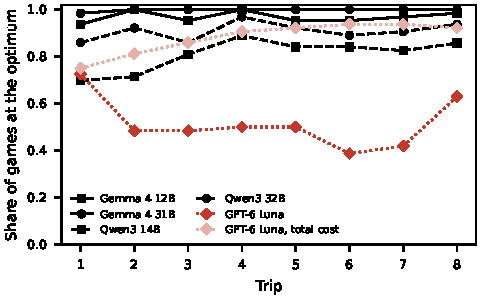
\includegraphics[width=\columnwidth]{generated/fig_so_by_trip}
\caption{Share of games at the optimum on each trip under the equality objective (shared messages, thinking on). Luna under total cost is shown for comparison.}
\label{fig:sotrip}
\end{figure}

\paragraph{Several answers.}
Luna agents write more plans than any open model (\RotLunaPlanners{} per game), often as complete trip-by-trip lists, but the lists differ between agents, and only \RotLunaSwap\% of groups swap to the complementary pair at the second trip (Table~\ref{tab:rotation}).

\paragraph{Recomputation.}
Once a trip goes off plan, Luna agents stop citing the earlier plan (\BreakPrecPre\% to \BreakPrecPost\% of first-round messages) and reassign by cumulative cost instead (\BreakTotPre\% to \BreakTotPost\%), for example ``give the R1 discount to the agent with the highest cumulative totals''. Rival assignments become more common (\BreakRivalPre\% to \BreakRivalPost\%), and a 2--2 split is declared by round 3 less often (\BreakConsPre\% to \BreakConsPost\%, against \BreakConsSocPost\% under total cost). A cost-based answer is unique only when two agents clearly lead: a 2--2 split is declared on \TieUniquePlan\% of such trips and on \TieTiedPlan\% when cumulative costs tie.

\paragraph{No commitment.}
Of \LunaFairTrips{} trips, \LunaFairFailed{} miss the optimum. Most of these failures, \LunaFairNoPlanFailed, occur on the \LunaFairNoPlan{} trips without a 2--2 split by round 3, where an average of \LunaFairNoPlanDev{} agents change route at the final choice and \LunaFairNoPlanSO\% of trips reach the optimum. Stable unanimous plans also break: someone deviates on \DefectLunaFair\% of \DefectLunaFairTrips{} such trips, against \DefectLunaSoc\% for Luna under total cost and at most \DefectGemmaMax\% for Gemma. In \DefectLunaFromCheap{} of \DefectLunaDev{} deviations the agent had declared the cheaper route. Luna does not return its reasoning, so we cannot tell why.

\paragraph{The cost of success.}
When coordination succeeds, the shared answer also decides who pays. Across fixed-role games of the open models, the pair p0, p1 holds the cheaper route in \FixedPairFront{} of \FixedPairGames{} (\FixedPairFrontPct\%), against one in six by chance, so the same positions bear the cost across independent groups.

\paragraph{Does it depend on sharing a model?}
All groups so far are monocultures. First-round messages already predict how mixed groups should behave. The probability that two independent first-round messages name the same assignment is \CoGG{} for two Gemma~4 31B agents, \CoLL{} for two Luna agents and \CoGL{} for one of each, but \CoQQ{} for two Qwen3 32B agents and \CoGQ{} for Gemma~4 31B with Qwen3 32B (total cost, route $A$ labelled R1). If agreement rests on a shared first answer rather than on identical weights, Gemma--Luna groups should coordinate about as well as homogeneous groups and Gemma--Qwen groups should not. \pending{Mixed-model groups (Gemma~4 31B with Luna, Gemma~4 31B with Qwen3 32B) and first-round probes that vary names and the wording of the equality sentence are planned.}

\section{Discussion and Conclusion}
\label{sec:discussion}
Groups of identical LLM agents solve the division problem of a congestion game quickly and without bargaining. Each agent writes an assignment for the whole group, and because the agents share a decision procedure, these independently written assignments tend to coincide; the exchange that follows confirms the result and later trips repeat it. Under an equality objective the same procedure writes a rotation schedule in the first message, a convention that human groups in comparable games reach only after hundreds of rounds \citep{helbing2005_turn_taking}.

This reverses the usual view of monoculture in one respect and confirms it in two. Shared priors let identical agents take different roles without negotiation, which work on independent decision makers would not predict \citep{ballestero2026_monoculture}. But when the shared answer is missing, failures are correlated, as when all agents switch together and overshoot \citep{kleinberg2021_monoculture}; and when the answer exists, it puts the cost on the same positions across groups \citep{bommasani2022_picking}.

The transcripts read like agreement, yet the agreement is a repeated derivation of the same answer rather than a commitment. No agent defends the interest of the user it would represent, and nothing in the protocol binds a declaration. Two practical implications follow for agents that share congestible resources. Rules that are easy to re-derive, such as a fixed schedule or a precedent, sustain coordination better than criteria recomputed on every trip. And expressions of agreement in multi-agent transcripts are weak evidence of negotiated consent; evaluations should report who bears the cost, not only how efficient the allocation is.

\section*{Limitations}
We study one four-agent, eight-trip congestion game, chosen because its optima are exact and efficiency and the division of cost separate cleanly; other games and larger groups may behave differently. The protocol uses simultaneous rounds with a mandatory declared route; sequential or free-form dialogue could change how agreement forms. All groups are homogeneous, and the mixed-model test is pending. Agent names and route labels are ordered and fixed. The message measures are lexical and structural, were designed after reading transcripts, and have so far been validated only by LLM coders. Reasoning traces, where available, are verbalized considerations and not faithful accounts of computation. Thinking mode is a stratum, not a randomized treatment. Luna returns no reasoning, is available only under an undated alias, and was run at two service tiers. No flagship closed model was tested. All prompts are in English. We make no claim about human behaviour or real traffic.

\section*{Ethics and Reproducibility}
All agents are simulated and no human data are collected. Model revisions, prompts, seeds, raw responses, reasoning traces where returned, execution settings, audits and analysis code are retained, and every number in this paper is generated from audited result files with recorded hashes. AI assistance was used for implementation and drafting.

\bibliography{refs}

\appendix
\section{Prompt}
\label{app:prompts}
For agent p0 on trip $t$, with R1 as route $A$ (labels swap in the paired game):
\begin{quote}\small\ttfamily
You are p0, one of 4 agents choosing between R1 and R2 over 8 trips. This is trip $t$.\\
R1 travel time is the number of agents choosing R1 on this trip divided by 4.\\
R2 travel time is 1.\\
{[}Objective sentence(s), if any.{]}\\
Each trip has 3 rounds for exchanging intended routes and messages, followed by simultaneous route choices.\\
Everyone receives all intended routes and messages after each round.\\
Past trips: {[}JSON{]}\\
Preparation records: {[}JSON{]}\\
Preparation round $k$ of 3. Return JSON with "intent" ("R1" or "R2") and "note" (text).
\end{quote}
With private messages, the two communication lines are replaced by ``Each trip has 3 rounds for privately recording your intended route and a note, followed by simultaneous route choices.'' The final call ends with ``Final choice. Return JSON with "route" ("R1" or "R2").'' \pending{Model revisions and sampling settings, full contrast tables, the lexicons and audit details to be added.}

\end{document}
